%%% This is file `elsarticle-template-1-num.tex',
%%
%% Copyright 2009 Elsevier Ltd
%%
%% This file is part of the 'Elsarticle Bundle'.
%% ---------------------------------------------
%%
%% It may be distributed under the conditions of the LaTeX Project Public
%% License, either version 1.2 of this license or (at your option) any
%% later version.  The latest version of this license is in
%%    http://www.latex-project.org/lppl.txt
%% and version 1.2 or later is part of all distributions of LaTeX
%% version 1999/12/01 or later.
%%
%% Template article for Elsevier's document class `elsarticle'
%% with numbered style bibliographic references
%%
%% $Id: elsarticle-template-1-num.tex 149 2009-10-08 05:01:15Z rishi $
%% $URL: http://lenova.river-valley.com/svn/elsbst/trunk/elsarticle-template-1-num.tex $
%%
\documentclass[preprint, 12pt]{elsarticle}
\usepackage{etoolbox}

\makeatletter
\patchcmd{\ps@pprintTitle}{\footnotesize\itshape
  Preprint submitted to \ifx\@journal\@empty Elsevier
  \else\@journal\fi\hfill\today}{\relax}{}{}
\makeatother

\usepackage{xpatch}

% Patching the \hrule\vskip12pt out .. do it twice!!!
\makeatletter
\xpatchcmd{\pprintMaketitle}{%
  \hrule\vskip12pt%
}{}{\typeout{Success}}{}

% Injection the date as a replacement of the 2nd `\hrule` stuff
\xpatchcmd{\pprintMaketitle}{%
  \hrule\vskip12pt%
}{\@date}{\typeout{Success}}{}
\makeatother

%% Use the option review to obtain double line spacing
%% \documentclass[preprint,review,12pt]{elsarticle}

%% Use the options 1p,twocolumn; 3p; 3p,twocolumn; 5p; or 5p,twocolumn
%% for a journal layout:
%% \documentclass[final,1p,times]{elsarticle}
%% \documentclass[final,1p,times,twocolumn]{elsarticle}
%% \documentclass[final,3p,times]{elsarticle}
%% \documentclass[final,3p,times,twocolumn]{elsarticle}
%% \documentclass[final,5p,times]{elsarticle}
%% \documentclass[final,5p,times,twocolumn]{elsarticle}

%% The graphicx package provides the includegraphics command.
\usepackage{graphicx}
%% The amssymb package provides various useful mathematical symbols
\usepackage{amssymb}
%% The amsthm package provides extended theorem environments
%% \usepackage{amsthm}

% for pdf outlines/bookmarks from section titles 
\usepackage[bookmarks,bookmarksopen,bookmarksdepth=3]{hyperref}
\hypersetup{pdftex,colorlinks=true,allcolors=blue}
\usepackage{hypcap}

% for bibi
% \usepackage{biblatex}

% for plotting diagrams by TKiz
\usepackage[latin1]{inputenc}
\usepackage{tikz}
\usetikzlibrary{shapes,arrows}
\usepackage{caption}
\newcommand*{\h}{\hspace{5pt}}% for indentation
\newcommand*{\hh}{\h\h}% double indentation


%% natbib.sty is loaded by default. However, natbib options can be
%% provided with \biboptions{...} command. Following options are
%% valid:

%%   round  -  round parentheses are used (default)
%%   square -  square brackets are used   [option]
%%   curly  -  curly braces are used      {option}
%%   angle  -  angle brackets are used    <option>
%%   semicolon  -  multiple citations separated by semi-colon
%%   colon  - same as semicolon, an earlier confusion
%%   comma  -  separated by comma
%%   numbers-  selects numerical citations
%%   super  -  numerical citations as superscripts
%%   sort   -  sorts multiple citations according to order in ref. list
%%   sort&compress   -  like sort, but also compresses numerical citations
%%   compress - compresses without sorting
%%
%% \biboptions{comma,round}

% \biboptions{}

\begin{document}

\begin{frontmatter}

  %% Title, authors and addresses

  \title{Using CMS Conference Schedules to Predict CMS Dataset Usage}

  \date{May 18, 2015}

  %% use the tnoteref command within \title for footnotes;
  %% use the tnotetext command for the associated footnote;
  %% use the fnref command within \author or \address for footnotes;
  %% use the fntext command for the associated footnote;
  %% use the corref command within \author for corresponding author footnotes;
  %% use the cortext command for the associated footnote;
  %% use the ead command for the email address,
  %% and the form \ead[url] for the home page:
  %%
  %% \title{Title\tnoteref{label1}}
  %% \tnotetext[label1]{}
  %% \author{Name\corref{cor1}\fnref{label2}}
  %% \ead{email address}
  %% \ead[url]{home page}
  %% \fntext[label2]{}
  %% \cortext[cor1]{}
  %% \address{Address\fnref{label3}}
  %% \fntext[label3]{}

  %% use optional labels to link authors explicitly to addresses:
  %% \author[label1,label2]{<author name>}
  %% \address[label1]{<address>}
  %% \address[label2]{<address>}

  \author[cs]{Ting Li (tl524@cornell.edu)}
  \author[phy]{Advisor: Valentin Kuznetsov (veknet@gmail.com)}

  \address[cs]{Computer Science Department, Cornell University}
  \address[phy]{Physics Department, Cornell University}
   

  
  % \address{Cornell University}

%  \begin{abstract}
    %% Text of abstract
%  \end{abstract}

\end{frontmatter}

%% main text
\section{Overview}
\label{S:1}

%% - problem statement
%% - your task goals

The Compact Muon Solenoid (CMS) is a large general-purpose particle physics detector, built on the Large Hadron Collider (LHC) at CERN in Switzerland and France. The goal of the CMS experiments is to investigate a wide range of physics, including the search for the Higgs boson, extra dimensions, and particles that could make up dark matter \cite{web:wiki}.
The CMS experiments present challenges not only in terms of the physics to discover and the detector to build and operate, but also in terms of the data volume and the necessary computing resources. Data sets and resource requirements are at least an order of magnitude larger than in previous experiments \cite{web:cms}.
The CMS computing system relies on a distributed infrastructure of Grid resources, services and toolkits, to cope with computing requirements for storage, processing and analysis of data provided by the experiments. 

It will be beneficial if we can reliably predict the usages of the datasets used in the future experiments, so the data management staff can make enough replicates of the datasets, and deploy them to the storage centers nearby, and thus increase the throughput of data delivery to the researchers. 

An approach to the prediction is to binarize the dataset access count in unit time (say, a week) into popularity labels, so that the problem becomes a classification one, and use the attributes from the CMS dataset access data as features \cite{web:vk}.
The approach can make sensible prediction in some experiments.
The IT engineers, however, are facing ever increasing demand of data delivery, so they continue on searching for ways to achieve better prediction performance.

My project task is to study if and how the CMS conference schedules can be useful for predicting CMS dataset future popularity.
This project is supervised by Valentin Kuznetsov. I thank him for his guidance and patience.


\subsection{Workflow and Design of the Project}

My modeling and analysis proceed in two directions:
\begin{itemize}
\item analyze the time series of the weekly conference count and the time series of the weekly access counts to each dataset,
\item evaluate weekly conference counts as new features added to the classification model.
\end{itemize}

The diagrams \ref{chart1} and \ref{chart2} are the flowcharts of the simplified processes in the two types of modeling and analysis in this project.
In the diagrams, program files are shown without being bounded by boxes, and the inputs, intermediates, and outputs of programs are shown inside boxes.
The inputs, intermediates, and outputs of a program are simplified, for example, there are much more dataset access files than the two shown for two weeks, and some programs also takes auxiliary inputs besides those shown in the diagrams.
The purpose of making the diagrams is to show the design and workflow of the project in a big picture.

% \documentclass{article}
%% \usepackage[latin1]{inputenc}
%% \usepackage{tikz}
%% \usetikzlibrary{shapes,arrows}
%% \usepackage{caption}
%% \newcommand*{\h}{\hspace{5pt}}% for indentation
%% \newcommand*{\hh}{\h\h}% double indentation
%% \begin{document}
\begin{figure}
\begin{center}
  % setting the typeface to sans serif and the font size to small
  % the scope local to the environment
  \sffamily
  \footnotesize
  \begin{tikzpicture}[auto, 
      %decision/.style={diamond, draw=black, thick, fill=white,
      %text width=8em, text badly centered,
      %inner sep=1pt, font=\sffamily\small},
      block_center/.style ={rectangle, draw=black, thick, fill=white,
        text width=10em, text centered,
        minimum height=4em},
      block_left/.style ={rectangle, draw=black, thick, fill=white,
        text width=16em, text ragged, minimum height=4em, inner sep=6pt},
      block_noborder/.style ={rectangle, draw=none, thick, fill=none,
        text width=12em, text centered, minimum height=1em},
      block_assign/.style ={rectangle, draw=black, thick, fill=white,
        text width=18em, text ragged, minimum height=3em, inner sep=6pt},
      block_lost/.style ={rectangle, draw=black, thick, fill=white,
        text width=16em, text ragged, minimum height=3em, inner sep=6pt},
      line/.style ={draw, thick, -latex', shorten >=0pt}]
    %
    % 1. outlining the flowchart using the PGF/TikZ matrix funtion
    \matrix [column sep=5mm,row sep=3mm] {
      % enrollment - row 1
      \node [block_center] (w1) {Dataset access records in week 1};
      & \node [block_center] (w2) {Dataset access records in week 2};
      & \node [block_center] (cf_dp) {Conference dump from database + schema}; 
      \\
      % enrollment - row 1'
      \node [block_noborder] (ts1) {\verb|time_series.py|};
      &
      & \node [block_noborder] (cf_parser) {\verb|cms_conf_parser.py|}; \\
      % enrollment - row 2
      \node [block_center] (ts2) {A dataset's access count per week time series};
      &
      & \node [block_center] (cf_ct) {Conference count per week time series}; \\
      % enrollment - row 2'
      \node [block_noborder] (ts31) {\verb|time_series.py|}; 
      & \node [block_noborder] (ts32) {\verb|time_series.py|}; 
      & \node [block_noborder] (ts33) {\verb|time_series.py|}; \\
      % enrollment - row 3
      \node [block_center] (result1) {Seasonality};
      & \node [block_center] (result2) {Cross correlation};
      & \node [block_center] (result3) {Seasonality}; \\
    };% end matrix
    %
    %
    % 2. connecting nodes with paths
    \begin{scope}[every path/.style=line]
      % paths for enrollemnt rows
      \path (w1)   -- (ts1);
      \path (w2)   -- (ts1);
      \path(ts1) -- (ts2);
      \path (cf_dp) -- (cf_parser);
      \path (cf_parser) -- (cf_ct);
      % 
      \path (ts2) -- (ts32); 
      \path (cf_ct) -- (ts32);
      \path (ts32) -- (result2);      
      \path (ts2) -- (ts31); 
      \path (ts31) -- (result1);
      \path (cf_ct) -- (ts33); 
      \path (ts33) -- (result3);
    \end{scope}
\end{tikzpicture}
\captionof{figure}{Flowchart of Time Series Generation and Analysis}
\label{chart1}
\end{center}
\end{figure}

% \end{document}

% \documentclass{article}
%% \usepackage[latin1]{inputenc}
%% \usepackage{tikz}
%% \usetikzlibrary{shapes,arrows}
%% \usepackage{caption}
%% \newcommand*{\h}{\hspace{5pt}}% for indentation
%% \newcommand*{\hh}{\h\h}% double indentation
%% \begin{document}
\begin{figure}
  \begin{center}
  % setting the typeface to sans serif and the font size to small
  % the scope local to the environment
  \sffamily
  \footnotesize
  \begin{tikzpicture}[auto, 
      %decision/.style={diamond, draw=black, thick, fill=white,
      %text width=8em, text badly centered,
      %inner sep=1pt, font=\sffamily\small},
      block_center/.style ={rectangle, draw=black, thick, fill=white,
        text width=10em, text centered,
        minimum height=4em},
      block_left/.style ={rectangle, draw=black, thick, fill=white,
        text width=16em, text ragged, minimum height=4em, inner sep=6pt},
      block_noborder/.style ={rectangle, draw=none, thick, fill=none,
        text width=12em, text centered, minimum height=1em},
      block_assign/.style ={rectangle, draw=black, thick, fill=white,
        text width=18em, text ragged, minimum height=3em, inner sep=6pt},
      block_lost/.style ={rectangle, draw=black, thick, fill=white,
        text width=16em, text ragged, minimum height=3em, inner sep=6pt},
      line/.style ={draw, thick, -latex', shorten >=0pt}]
    %
    % 1. outlining the flowchart using the PGF/TikZ matrix funtion
    \matrix [column sep=5mm,row sep=3mm] {
      % enrollment - row 1
      \node [block_center] (w1) {Dataset access records in week 1};
      & \node [block_center] (cf_dp) {Conference dump from database + schema};
      & \node [block_center] (w2) {Dataset access records in week 2}; \\        % enrollment - row 1'
      \node [block_noborder] (split1) {\verb|select.py|};
      & \node [block_noborder] (cf_parser) {\verb|cms_conf_parser.py|}; 
      & \node [block_noborder] (split2) {\verb|select.py|}; \\
      % enrollment - row 2
      \node [block_center] (w1_ti) {Access records for datasets in some tier};
      & \node [block_center] (cf_ct) {Weekly conference count time series}; 
      & \node [block_center] (w2_ti) {Access records for datasets in some tier}; \\
      % enrollment - row 2'
      \node [block_noborder] (merge_acc_conf1) {\verb|merge_access_conf.py|};
      & 
      & \node [block_noborder] (merge_acc_conf2) {\verb|merge_access_conf.py|}; \\
      % enrollment - row 3
      \node [block_center] (w1_cf) {Dataset access + conference count};
      & 
      & \node [block_center] (w2_cf) {Dataset access + conference count}; \\
      % enrollment - row 3'
      & \node [block_noborder] (merge_dfs) {\verb|merge_csv.py|}; 
      & \\
      % follow-up - row 4
      & \node [block_center] (w12) {Week 1 and 2 combined};
      & \node [block_noborder] (same1) {... ...}; \\
      % enrollment - row 4'
      & \node [block_noborder] (transform) {\verb|transform_csv.py|}; 
      & \node [block_noborder] (same2) {\verb|transform_csv.py|};  \\
      % follow-up - row 5
      & \node [block_center] (trainset) {Train set (some cols dropped, outcome binarized)};
      & \node [block_center] (testset) {Test set (some cols dropped, outcome binarized)}; \\
      % follow-up - row 5'
      & \node [block_noborder] (model) {\verb|model.py|};
      & \\
      % follow-up - row 6
      & \node [block_center] (classifier) {Classifier + feature ranking + predictions on test set};
      & \\
      % follow-up - row 6'
      & \node [block_noborder] (check_pred) {\verb|check_prediction.py|};
      & \\
      % follow-up - row 5
      & \node [block_center] (test_perf) {Test performance};
      & \\
    };% end matrix
    %
    %
    % 2. connecting nodes with paths
    \begin{scope}[every path/.style=line]
      % paths for enrollemnt rows
      \path (w1)   -- (split1);
      \path (split1)   -- (w1_ti);      
      \path (w2)   -- (split2);
      \path (split2)   -- (w2_ti);      
      \path (cf_dp) -- (cf_parser);
      \path (cf_parser) -- (cf_ct);
      % 
      \path (w1_ti) -- (merge_acc_conf1); 
      \path (cf_ct) -- (merge_acc_conf1);
      \path (merge_acc_conf1) -- (w1_cf);     
      \path (w2_ti) -- (merge_acc_conf2);
      \path (cf_ct) -- (merge_acc_conf2);            
      \path (merge_acc_conf2) -- (w2_cf);      
      %
      \path (w1_cf) -- (merge_dfs);
      \path (w2_cf) -- (merge_dfs);
      \path (merge_dfs) -- (w12);
      \path (same1) -- (same2);      
      %
      \path (w12) -- (transform);
      \path (transform) -- (trainset);
      \path (same2) -- (testset);
      %
      \path (trainset) -- (model);
      \path (testset)  -- (model);
      %
      \path (model) -- (classifier);
      \path (classifier) -- (check_pred);
      \path (check_pred) -- (test_perf);      
    \end{scope}
  \end{tikzpicture}
\captionof{figure}{Flowchart of Classification and Train/Test Set Generation}
\label{chart2}
\end{center}
\end{figure}
% \end{document}


The programs which I have written are the following. They are written in Python, and run under \verb|Python| 2.6.8 on 64-bit Scientific Linux CERN 6 (SLC6) on the \verb|lxplus.cern.ch| server \cite{web:lxplus}. I made them  available on GitHub \cite{web:tlgithub}. Here I include brief descriptions of the programs:

\begin{itemize}
\item \verb|cms_conf_parser.py|
  
  It parses the conference data dump file into a conference count time series.

  Input:

  \verb|--indump|: a csv.gz file for conference data dump from a database

  \verb|--inschema|: a plain text file for the schema of the conference data dump file

  Output:

  \verb|--outdir|: a directory containing  a csv.gz file for the output weekly conference count time series, a csv.gz file for the output conference counts up to some future weeks, and a csv.gz file for the output parsed conference records
  
  
\item \verb|select.py|

  It selects records from dataset access files whose attribute has some value.

  Input:
  
  \verb|--indir|: a directory containing the csv.gz files for the input dataset access data

  \verb|--attr|: an attribute to select by

  \verb|--attrval|: a value of the attribute to select by

  Output:

  \verb|--outdir|: a directory containing csv.gz files for the output selected records

\item \verb|merge_access_conf.py|

  It add records from conference counts to dataset access records

  Input:

  \verb|--indir|: a directory containing the csv.gz files for the input dataset access data

  \verb|--inconf|: a csv.gz file for the input weekly conference count data

  Output:

  \verb|--outdir|: a directory containing csv.gz files for the output merged data 

\item \verb|time_series.py|

  It generates time series for each dataset from the dataset access data, and analyze the cross correlations and seasonalities for the time series of dataset access and time series of conference count.

  Input:
  
  \verb|--indir|: a directory containing csv.gz files for the input dataset access data

  \verb|--inconf|: a csv.gz file for the input weekly conference count data

  Output:

  \verb|--outdir|: a directory containing csv.gz files for the output time series of each dataset, and image files for the plots of cross correlation and FFT of the time series

\end{itemize}


The other programs shown in the flowcharts were written by Valentin \cite{web:vkgithub}, which are part of package \verb|DCAFPilot| (version 0.0.42). I slightly modified his \verb|model.py| for  adding independence tests between each feature and the outcome, changing the split ratio of train and validation sets, fixing the random seeds, and changing the number of feature in the feature importance output.

\section{Preparing Datasets}
\label{S:2}
% - produced dataset (how you generate it and where it is stored)

\subsection{CMS Conference Data}


I receive the CMS conference data in a file, which was dumped from querying a database.
It contains a collection of conference records.
Each record represents a conference, and consists of the conference's ID, name, category, description, held time, held location, website link, etc.

I perform the following processings on the conference data dump file, to generate the data needed for modeling and analysis:

\begin{itemize}
  
\item In the conference data file, each record occupies multiple lines, and records are separated by a blank line, the fields of a record are separated by a comma or a new line, and each field may have comma(s) inside or may even be empty (that is, missing).
Thus we need to  Parse the text in the conference data file, into a list of dictionaries in Python, with each dictionary representing a conference record.
I perform the parsing according to the conference records' schema, which provide each attribute's name, type, and length when it is the string type.
The parsing of the dump file according to the schema is implemented by regex pattern matching in \verb|cms_conf_parser.py|.

\item After parsing, we count the conferences that are held in each week, and obtain a time series of weekly conference count over the weeks from the beginning of 2006 to mid September 2015 (505 weeks in total).  
This is implemented in \verb|cms_conf_parser.py|, by grouping the conference records by week, which is in turn implemented by creating a dictionary, with a key being a week, and its value being a list of conference records falling into that week.
Note that a week here is not a calendar year. The first day of a year is always the start of the first week of the year, and the last week of a year may contain more than 7 days.

\end{itemize}


\subsection{CMS Dataset Data}

I receive the CMS dataset data as a collection of files.
Each file stores the records of datasets accessed in a week. In such a file, each record is for a dataset, and the fields of a record are the information about the record's dataset (such as its id, size) and the usage of the dataset during the file's week (such as number of its accesses and cpu time of its accesses in the week). \cite{web:vk} has explanations for the attributes of the records.
The timestamp week for a file is not in the file's content, but is coded in the file's name, for example, \verb|dataframe-20130101-20130107.csv.gz|.

The files are easier to parse  than the files for conference data, because their contents are organized in a csv file format: 
each record occupies a line, the records are separated by a newline character, and the fields of a record are separated by a comma.

I perform the following processings on the dataset access files, to generate the data needed for modeling and analysis:

\begin{itemize}
  
\item Select records for datasets belonging to a tier.
This is implemented by list comprehension in \verb|select.py|.
Tiers are levels in the hierarchy of CMS distributed computing infrastructure. 
There are certain tiers whose sites store datasets dedicated to software testing, and the access to those datasets is unrelated to their access by physicists. Thus those  datasets are of little interest to our project, and we focus only on datasets from Tier 2 (reconstructed data) and Tier 3 (analysis data).
In this report, the datasets used for analysis and modeling come from Tier 2, and modeling and analysis for datasets from Tier 3 are similar.

\item For each dataset, group its records from all the dataframe files, and extract weekly dataset access count and output a time series of weekly access count over the weeks when the dataset has records.
This is implemented in \verb|time_series.py|.
The grouping is implemented by using a dictionary, with each key being a dataset and its value being a list of the records of the dataset.
For a record, the dataset it belongs to is identified by the \verb|dataset| and \verb|dbs| attributes,
and the access count to the record's dataset in the record's week is the value of the \verb|naccess| attribute.


\end{itemize}

\subsection{Add Conference Counts to Dataset Access Records in the same week}

For modeling the problem as a classification one in a later section, we merge the conference data to the dataset data.
To each dataset access record, I add the following new fields: the conference counts in the same week as the dataset access record, and the accumulated conference counts up to some future weeks.
This needs to find the corresponding conference count for a given week, which is implemented by matching the timestamp of a dataset access record to the timestamp of a conference count, again a string pattern matching problem.
This is implemented in \verb|merge_access_conf.py|.

\section{Time Series Analysis}

%% - plots confirming the study
%% - metrics you choose
%% - description of analysis
%% - analysis results


As mentioned in the Overview section,
my task is to study whether and how conference data can be used, possibly with CMS dataset data, for predicting future dataset usage.
My study has been going in two directions, which differ in whether and how we take into account the timestamps of the CMS dataset records and of conference schedules.

In the first direction, I analyze the relation between two time series: the weekly conference count, and an individual dataset's weekly access count.

Note that:

\begin{itemize}

  \item
There are 3279 datasets in Tier 2, but I do not consider them all for the following reasons.

Different datasets have different numbers of records.
For time series analysis purpose, I only consider those datasets which have more than $10$ records. There are $237$ of them.
The maximum length of a dataset is $103$, the minimum is $1$, and the median is  $5$, and the standard deviation is $5.59$.
The histogram of dataset lengths is in Figure \ref{len}.
 
\begin{figure}
\begin{center}
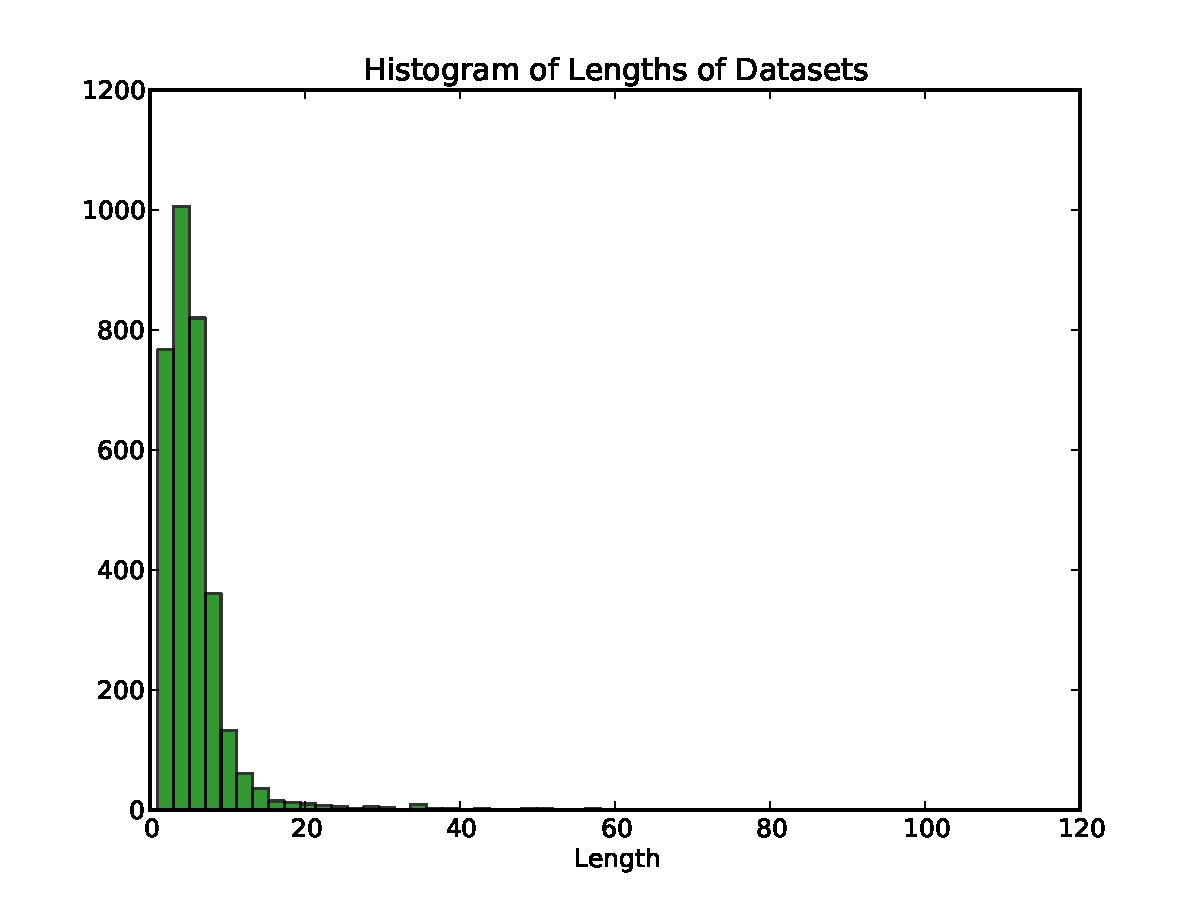
\includegraphics[scale=0.5]{../data/timeseries/datasets/dataset_3279_lengths_hist.pdf}
\end{center}
\caption{Histogram of lengths of dataset access count series}
\label{len}
\end{figure}
   
 
The \verb|naccess| attribute of some datasets are constant (for example, $0$), which makes cross-correlation become invalid, and Fourier transform to be a single spike at frequency $0$. Prediction of \verb|naccess| of such datasets is also trivial. Therefore I remove such datasets.
There are $2973$ datasets whose \verb|naccess| attributes are constant, and $2959$ of them are constantly $0$.
The maximum, minimum, median and standard deviation of variances of \verb|naccess| attribute values among the datasets are $826207739.67, 0, 0$, and $22326593.86$.

After filtering datasets by the above two criterions, $125$ datasets remain for the time series analysis.

\item
The records of a dataset can be missing for some weeks between its existing records in other weeks. For the purpose of time series analysis, I deal with the missing values by filling with $0$ for \verb|naccess| in missing weeks.

\end{itemize}

\subsection{Seasonality}

It is our original guess that conference schedules and dataset access may expose seasonalities or periodicities, due to holidays and vacations.
If it were true, we then would like to use their seasonalities or periodicities to simplify our modeling.

It is not obvious to identify seasonality in either the plot of the conference count series  or an arbitrary dataset access series however.
An alternative way to study seasonality in a time series is to calculate discrete Fourier transform on the time series by the fast Fourier transform algorithm, and search for significant spikes that represent the frequencies of seasonalities.
I calculate the FFT of a time series using numpy.fft.rfft().
Existence of noises in a time series usually leads to spurious spikes in its DFT series. Picking out the highest spikes requires smoothing the series with trial and error.
Thus I prefer visually checking over automatically choosing the highest spikes.


Figure \ref{cffft} is the plot of the DFT of the conference count series, and  \ref{dsfft1} and \ref{dsfft2} the DFT of some datasets' access count series.

\begin{figure}
\begin{center} 
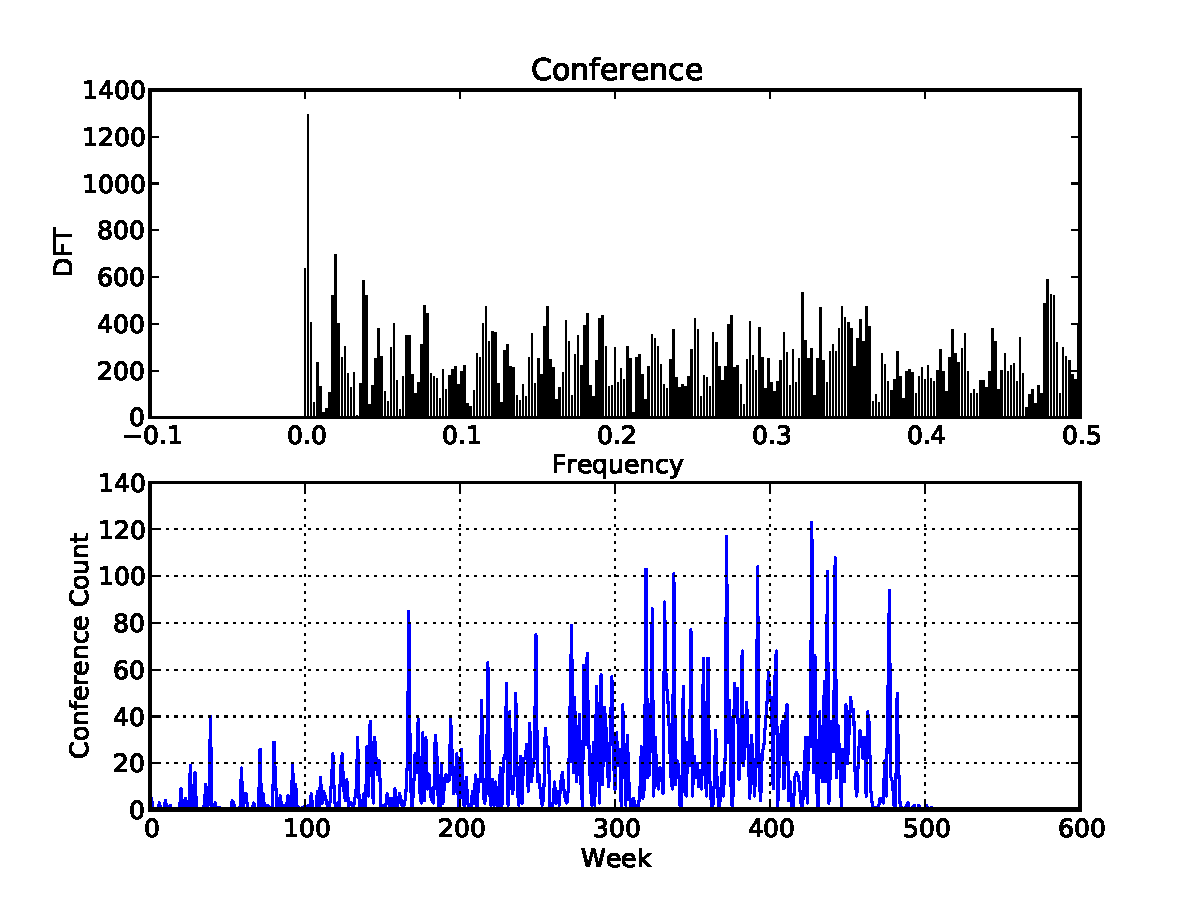
\includegraphics[scale=0.5]{../data/timeseries/datasets/conf_ct_perweek_505fft.pdf}
\end{center}
\caption{DFT of weekly conference count time series}
\label{cffft}
\end{figure}

In the DFT plot \ref{cffft} of the conference count series, the highest spike occurs at the first frequency (that is, frequency $1/505$, where $505$ is the length of the time series in weeks) , which does not imply periodicity, because it corresponds to the whole time domain of the time series ($505$ weeks from the beginning of 2013 to the middle of September 2015). The second highest spike occurs at the 10th frequency (that is, frequency $10/505$), which corresponds to a time period of $505/10 = 50.5$ weeks, roughly a year. This confirms our initial guess of seasonality due to holidays. Since the spike at the first frequency is so dominant, and the second highest spike is not much higher than the other spikes, the time series itself exhibit only slightly periodicity from the second highest spike.

\begin{figure}
\begin{center}
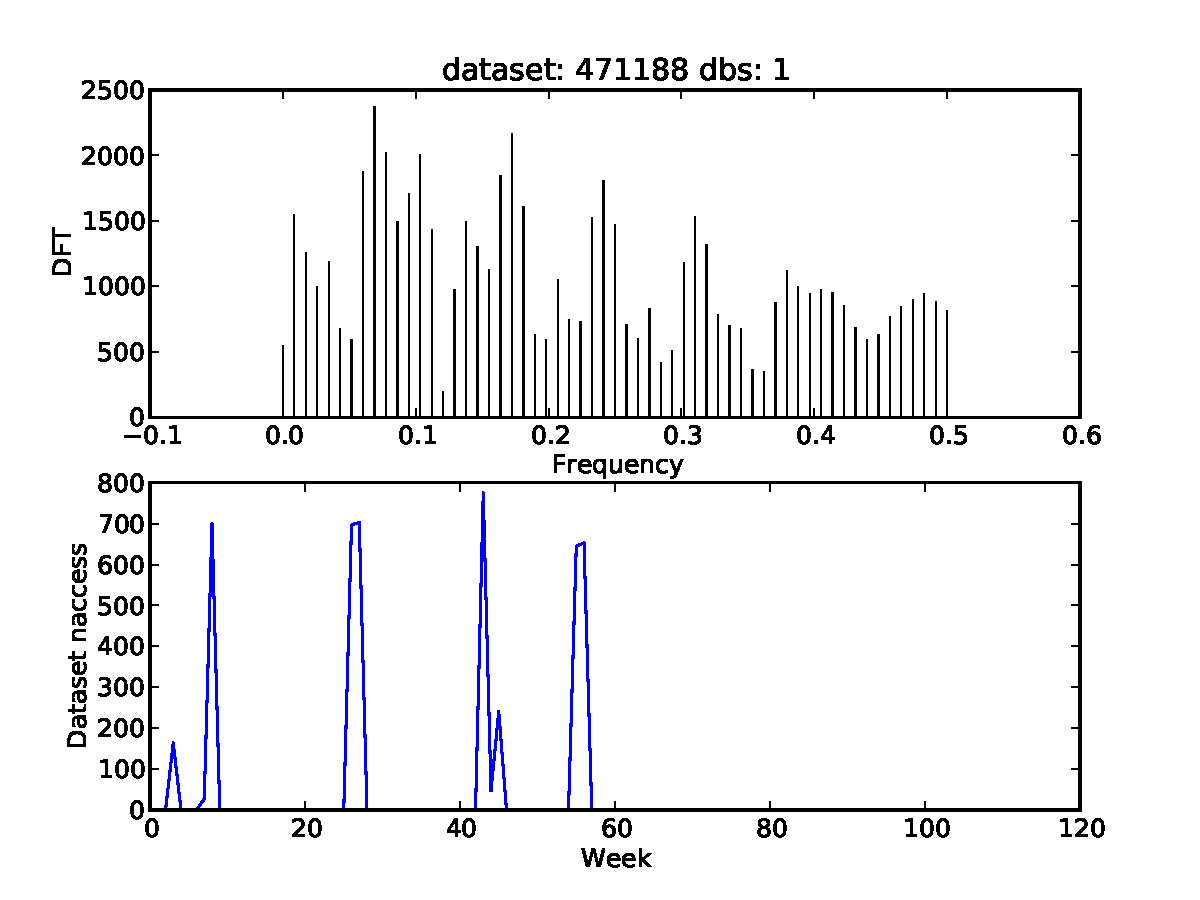
\includegraphics[scale=0.5]{../data/timeseries/datasets/471188_1_116_fft.pdf}
\end{center}
\caption{DFT of weekly access count time series  of a dataset}
\label{dsfft1}
\end{figure}


In the DFT plot \ref{dsfft1} of the access series of the dataset (471188,1), the highest spike occurs at the 8th frequency (that is, frequency $8/116$, where $116$ is the length of the time series in weeks), which corresponds to a time period of $116/8 = 15$ weeks. This coincides with the observation of a periodicity between 10 and 20 weeks from the plot of the time series itself.

\begin{figure}
\begin{center}
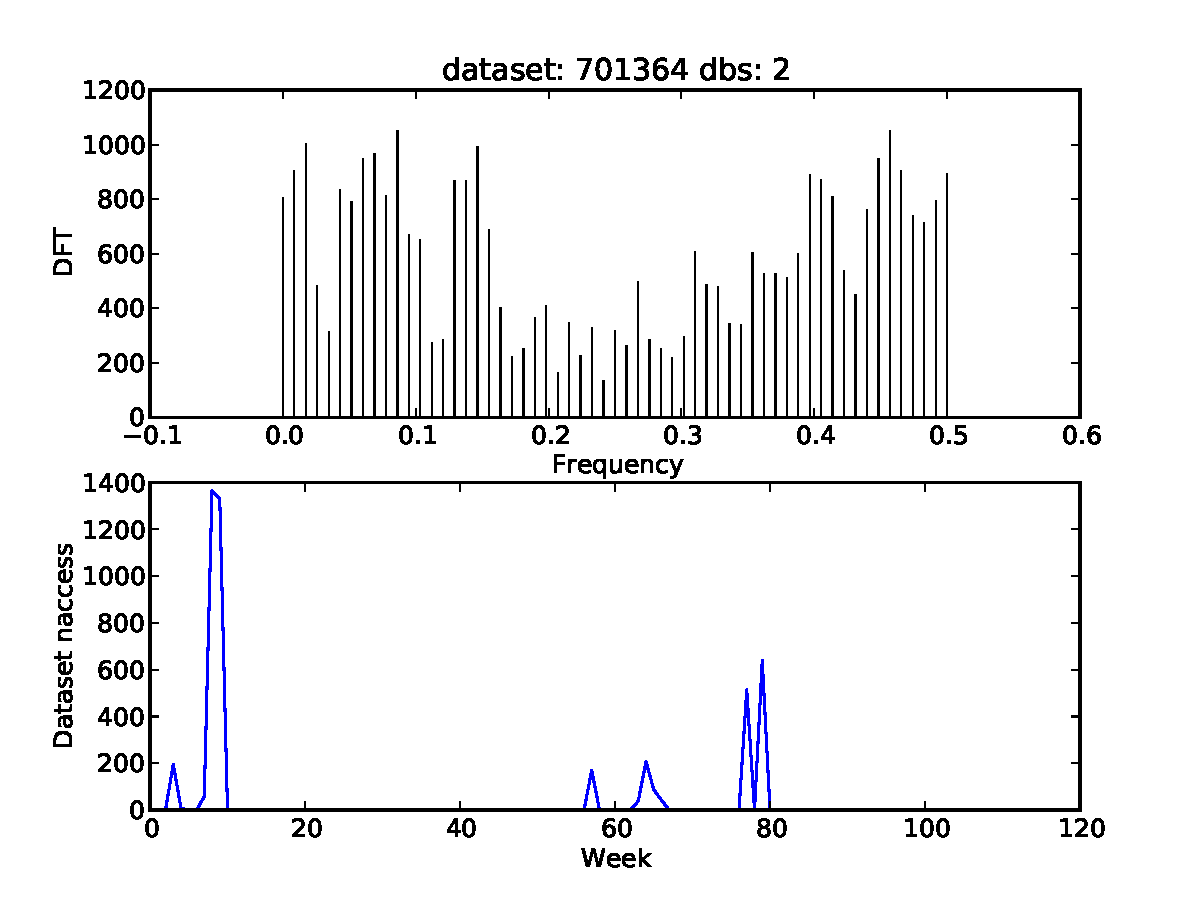
\includegraphics[scale=0.5]{../data/timeseries/datasets/701364_2_116_fft.pdf}
\end{center}
\caption{DFT of weekly access count time series of a dataset}
\label{dsfft2}
\end{figure}


In the DFT plot \ref{dsfft2} of the access series of the dataset (701364,2), there is no spike significantly higher than the others. So there seems no significant seasonality in the dataset access series.

The DFT plot varies from dataset to dataset, and there seems not guarantee to find seasonality in them.

Neither is it clear yet how to relate the seasonalities of the dataset access series with that of the conference count series.
If both the conference count series and an individual dataset access count series are both periodic,
we may limit our study to a time interval whose length is the common least multiple of their periods, instead of the entire time intervals where the two time series were created/defined.


\subsection{Cross Correlation}

I calculate the cross correlation between  an individual dataset's access count series and the conference count series, over lags ranging between $-90$ and $90$ with step $1$. At each lag, I call \verb|scipy.stats.stats.pearsonr()| to calculate a cross correlation, and besides a cross correlation, it also returns a p-value for testing a null hypothesis that the two series are uncorrelated at the lag.

The plots \ref{cor1}, \ref{cor2} and \ref{cor3} are the cross correlation between the access count series of some exemplar datasets and the conference count series.

\begin{figure}
\begin{center}
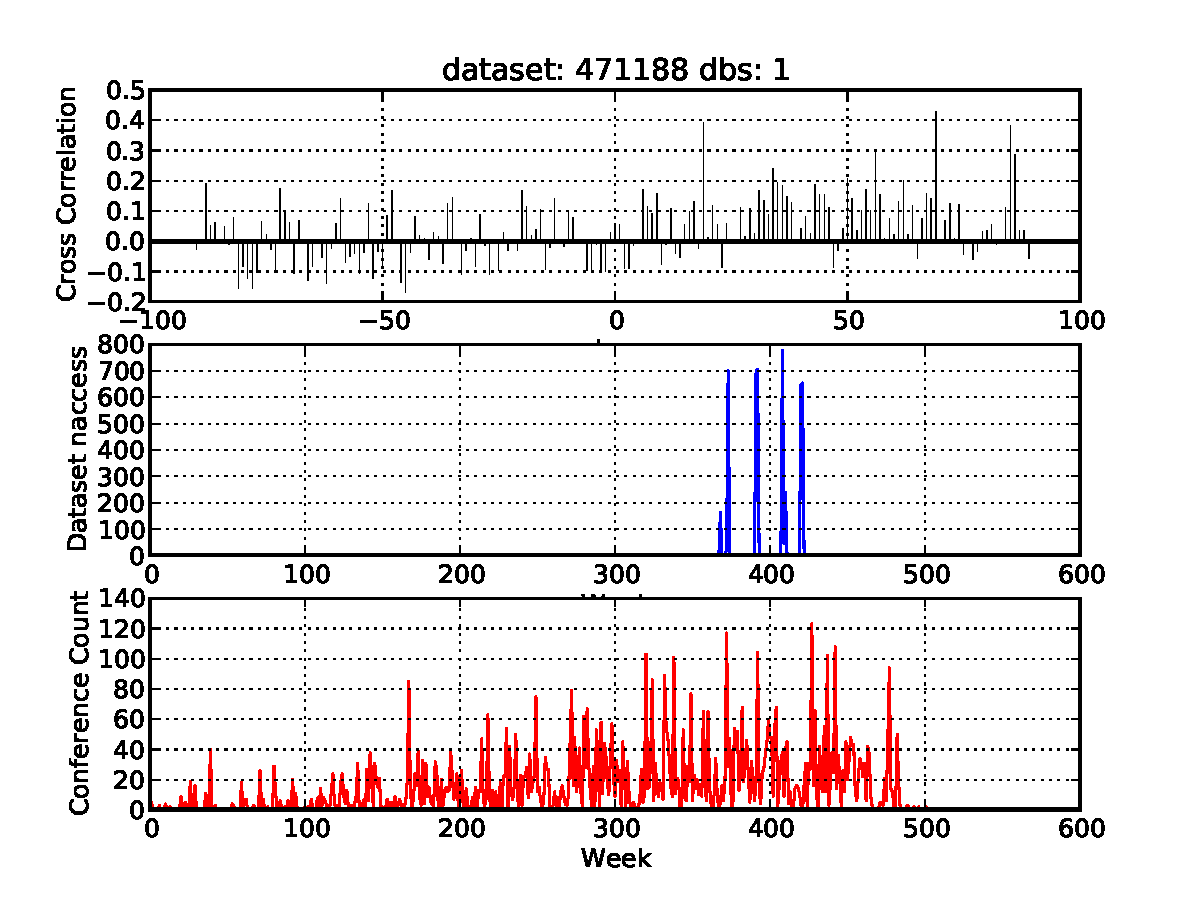
\includegraphics[scale=0.5]{../data/timeseries/datasets/471188_1_365.pdf}
\end{center}
\caption{Cross correlation between the conference count series and the access count series of a dataset}
\label{cor1}
\end{figure}

\begin{figure}
\begin{center}   
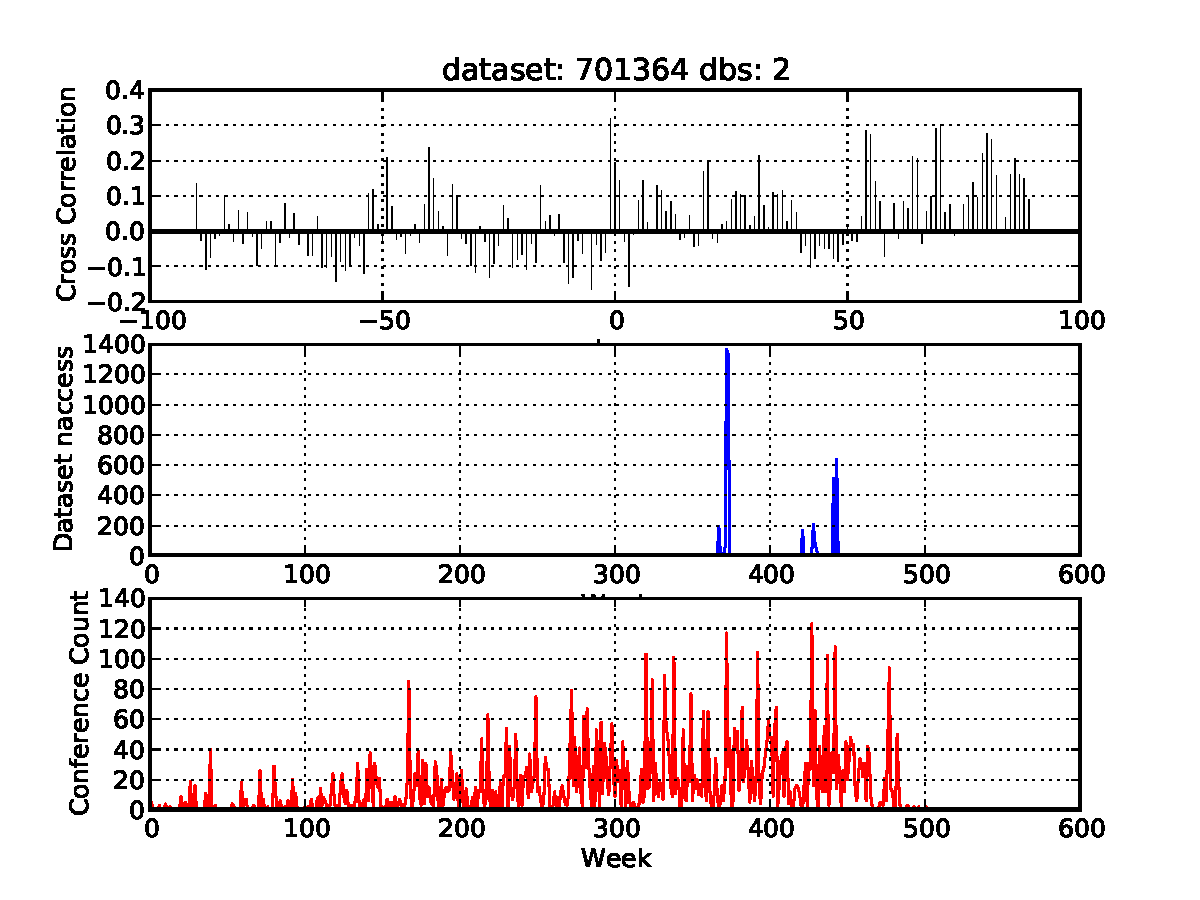
\includegraphics[scale=0.5]{../data/timeseries/datasets/701364_2_364.pdf}
\end{center}
\caption{Cross correlation between the conference count series and the access count series of a dataset}
\label{cor2}
\end{figure}

\begin{figure}
\begin{center}
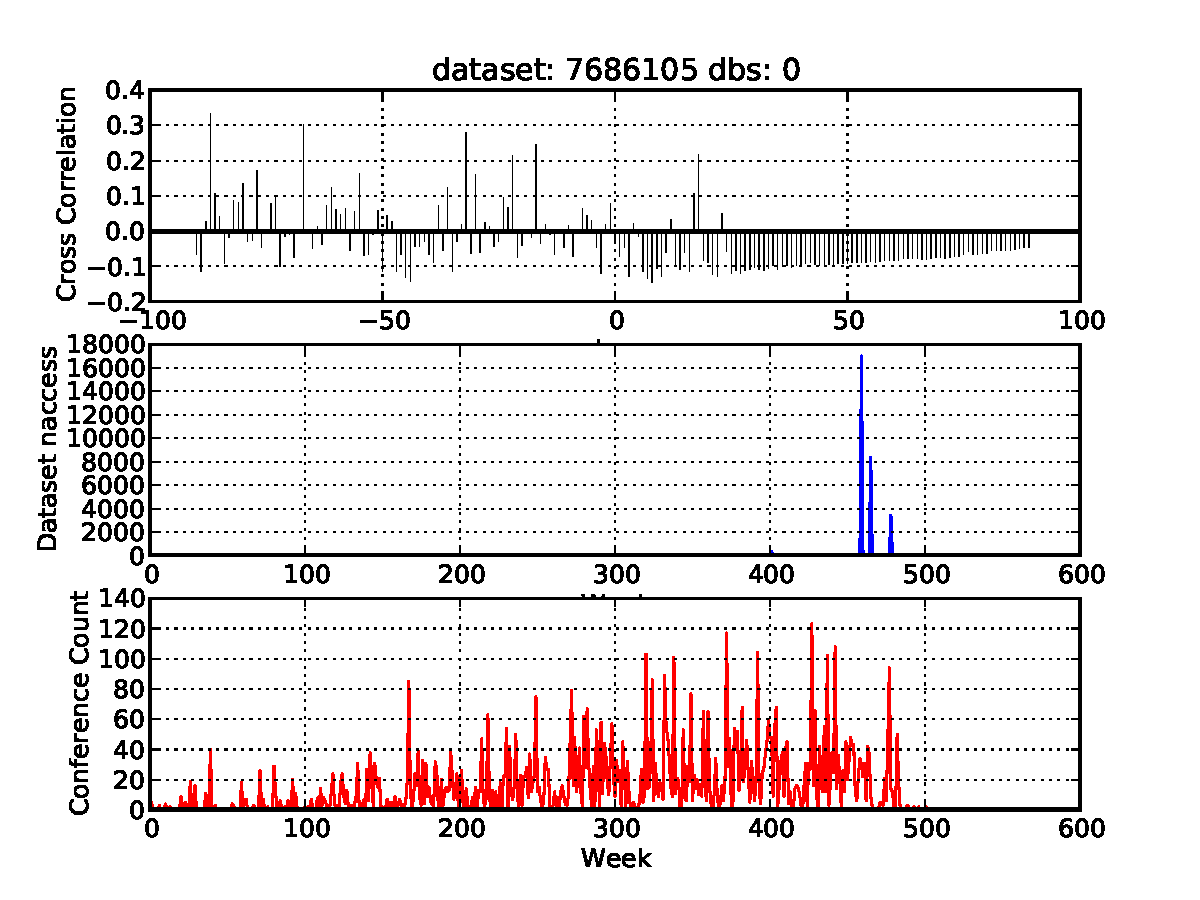
\includegraphics[scale=0.5]{../data/timeseries/datasets/7686105_0_372.pdf}
\end{center}
\caption{Cross correlation between the conference count series and the access count series of a dataset}
\label{cor3}
\end{figure}


The plots show that the lag where the highest cross correlation in magnitude occurs varies with different datasets, and can be either positive lags (for example, the plot for datasets \verb|(471188,1)| and \verb|(701364,2)|), or negative lags (for example, the plot for dataset \verb|(7686105,0)|).
Cross correlation peaking at a positive lag means that future conference schedules can lead the current dataset access, while peaking at a negative lag means that past conferences can still have residual influence on the current dataset access.


The plot \ref{laghist} is the histogram of such lags with p-values smaller than 0.05 (indicating the uncorrelated null is rejected with significance level 0.05). It shows that cross correlation achieves its maximum most probably around $75$ lags in weeks (roughly one year and a half), and with decreasing frequencies at the lags  $65, 85, 40, 50, 60$, and $5$:
 
\begin{figure}
\begin{center}
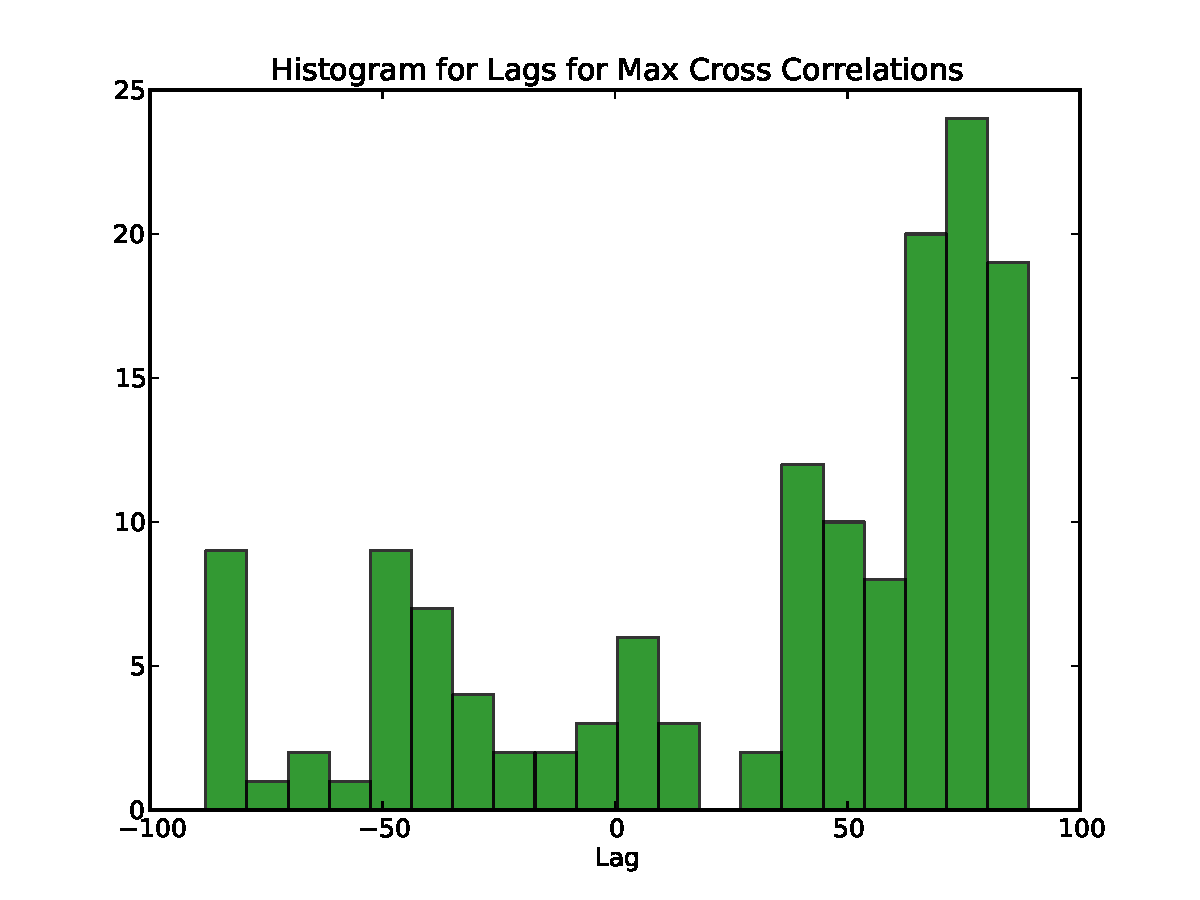
\includegraphics[scale=0.5]{../data/timeseries/datasets/lag_144_hist.pdf}
\end{center}
\caption{Histogram of lags with maximum cross correlation}
\label{laghist}
\end{figure}

For a given dataset, we can build a prediction model, by regressing the dataset weekly access count on conference counts in some future weeks away by the lags chosen from the cross correlation analysis.
There are potential drawbacks of such modeling:

\begin{itemize}
  
\item We assume the relation between dataset access count and future conference counts are the same over the time, which is something like or similar to stationarity: the distribution of the dataset weekly access count given the future weeks' conference counts is the same across the weeks. After building such models, we lose track of time.
Without the stationary assumption, it remains to build a forecast model that can capture the nonstationarity in the relation between the two time series.
In any case, it will be good to test if the stationary assumption holds up front.

\item It does not make use of the other attributes from CMS dataset data, except using the dataset access count as the outcome.

\end{itemize}

\section{Classification}

In this section, we consider a different direction from time series analysis.

We simplify the quantitative outcome, that is, the weekly dataset access count, to a qualitative popularity class label, by binarizing the counts at a threshold 100.
% choose threshold for output target? by seeing histogram of the output target in train set, and by requirement such as how much percentage of dataset should be positive at a time (not necessarily 50%) (since he set it to be 100, there must be a reason? so don't change the threshold?)? 
% threshold is fixed for  all weeks, because popularity criterion is same for all weeks.
This changes the problem from a regression one to a classification one, potentially increasing the generalization ability of the trained model.
% try regression instead of classification?
% is the high dim of features may be a problem more to regression than to classification? but for random forest regressor?

Moreover, we make the following stationary assumption:
within a certain period, the conditional distribution of the dataset popularity binary outcome on the features (that is, future conference counts and other dataset attributes from CMS dataset data, see below) changes little over time, and can be approximately seen as being stationary.
So we drop the timestamps from the data after combining the conference counts and the dataset access records.
For example,
we assume the length of such a period can be around one year (about 52 weeks), and choose to train on the data from the May 2013 to April 2014, and test on the data in the following week after April 2014.

 
% - Assume all the datasets follow the same model. So we further drop the dataset id (\verb|dataset|, \verb|dbs|).
% he uses dataset id as features (categorial features) for training RF classifier.

\subsection{Candidate Features}

When choosing the candidate features to be considered in the classification problem, I would like to consider all that are available, and might later perform feature selection as needed.

The candidate features are the future conference counts weeks away by lags chosen from the cross correlation analysis of time series, and the attributes in CMS dataset data that are available at the time of prediction.

We consider the future conference counts as candidate features, because we suspect that the future conference schedules may influence current dataset access counts, and they are available for predicting accesses to the datasets.

Not all attributes from the dataset access records have their values available before the time to predict for.
For example,
\verb|naccess| is what we generate the binary outcome directly from, so it must obviously be dropped.
So are \verb|nusers| (the number of users $*$ days to a dataset, reported by PopularityDB), and \verb|totcpu| (the number of cpu hours to accessed dataset, reported by PopularityDB).
Valentin  singled them out in his demo examples of using his programs \cite{web:vk}.
% manual feature selection, which depends on relation to outcome:
% does cpu and proc_events relate to naccess, and should be dropped? they both have high importance in random forest.
% id is dropped because specified as id to model?
% dataset and dbs are both categorical, and useful for classifying popular and unpopular.

The weekly conference count can change dramatically, so instead of using them directly, I use more stable features which are the accumulated future conference counts up to $1, 2, 4, 6, 10, 15, 20, 25, 30, 35, 40, 45, 50, 55, 60, 65$, and $70$ weeks. The number of the weeks are chosen somehow based on the lags at which the cross correlation between conference count series and dataset access count series is high (see the previous section).


\subsection{Feature Types}

Classifier, feature transformation, feature selection and ranking may work with some feature types (categorical, ordered, numerical, ...), and not with other feature types.

Some features from CMS dataset data seem to be categorical, for example, \verb|dataset|, \verb|dbs|, and \verb|rel*|.
In the dataset access files, however, all the features (including categorical ones) are coded in numerical values.
This can be problematic if not handled correctly.
  
Decision trees and therefore random forest can take categorical features. %esplly for binary outcome, c.f. hastie $9.2.4
Scikit-Learn does not directly support categorical features in trees or forests however \cite{web:slcat}. % how to specify a feature is categorical instead of numerical to scikit learn algorithms?
If categorical features are coded as numbers, which imposes a non-existing ordering on the categorical values,
the random forest training algorithm will rely on that ordering,  and the trained random forest classifier will be misleading in terms of interpretation and have more overfitting to the training data.
% Feature importances calculated in random forest classifier may not work for numerically coded categorical features?

It may also be misleading to apply numerical feature transformation (such as standardization of features  to have zero mean and unit variance) on  categorical features that are numerically coded.
The random forest training algorithm theoretically does not depend on standardization, because standardization does not change the ordering between the feature values.
If we use random forest for classification, it seems better not to do standardization in preprocessing. (When I set  \verb|scaler=None| (or just not specify the option) to the program \verb|model.py|, the program will not predict on the test set.)
% Q: how to pass none to scaler. in "model.py", there is a test "if opts.scaler". 


\subsection{Ranking Sets of Features}

We can compare different sets of features, by using them to train classifiers, and comparing the classifiers' test performances.
Here I train random forest classifiers by calling \verb|model.py|, which in turn calls the learning algorithm implemented in the Scikit-Learn library by the class \verb|sklearn.ensemble.RandomForestClassifier|.

We are interested more in the popular class (that is, the positive class) than the unpopular one (that is, the negative class), so we choose classification performance measures that more focus on the positive class:  accuracy, precision, recall and $F1$ scorers.

Note:

\begin{itemize}
  
\item I use the default complexity settings of a random forest classifier based on the empirical recommendations in the library's user guide.
In the default settings,
a random forest has 10 random trees, 
each tree is allowed to be constructed without constraints on its complexity (depth), and
the number of the candidate features randomly chosen at each node split is the square root of the number of all the features.

Thanks to the randomization in constructing each tree, and the averaging of the probabilistic predictions of all the trees, 
the tendency of a random forest classifier to overfit is generally small. % more immune to curse of dimensions, that is, can work with  many features?
Thus I skip the validation step to tune the complexity of the forest, and then the usage of validation set is not necessary.
Also because validation reduces the actual training set, I skip validation by setting the validation set's percentage \verb|split=0| in \verb|model.py|.

\item To make the experiments reproducible, I fix the random seeds in the program \verb|model.py|, which appear in
the \verb|random_state| parameter to both the forest constructor function \verb|sklearn.ensemble.RandomForestClassifier()|, and to the splitting dataset function \verb|train_test_split()|.
Since I skip validation by setting the validate size \verb|split=0|,  the \verb|random_state| parameter to  \verb|train_test_split()| does not matter.
% the output is random, although the random_state parameter is set to be fixed in model.py "setattr(clf, "random_state", 123)". why?
% he miss the random_state param for  train_test_split(). 

\end{itemize}


% I modify model.py to output importance for all features, not just the first 9 most important features


%% \subsubsection{}

%% - compare the classification performances with different sets of features

%% train a random forest classifier with different sets of features, and compare them more easily?
%% - conferent counts alone (with dataset id  (dataset, dbs) from CMS dataset data, which I want to skip but don't figure out how to in the program \verb|model|)
%% - the attributes in CMS dataset data.
%% - combination of all the above features.

\subsection{Ranking Individual Features}

There are different ways to rank individual features in a classification problem.


\subsubsection{Importance Measurements Returned by Random Forest Classifier}
% instead of using random forest,  check if conf count is related or important to the classification or regression, by some other ways?

When a random forest classifier make predictions on a test set,
the relative rank (that is, depth) of a feature used as a decision node in a tree can be used to assess the relative importance of that feature with respect to the predictability of the target variable. Features used at the top of the tree contribute to the final prediction decision of a larger fraction of the input samples. The expected fraction of the samples they contribute to can thus be used as an estimate of the relative importance of the features. \cite{web:slguide}

Note that a random forest classifier trained from a train set has already arranged the features at each node based on the train set, so the calculation of feature importance by the trained random forest classifier should be on a different data set (here a test set).

In an object of the class \verb| sklearn.ensemble.RandomForestClassifier|, the attribute \verb|feature_importances_| stores the importances of the features on a test set.

\subsubsection{Feature Ranking by Independence Testing}

Alternatively, we can rank the features, by testing the independence between each feature and the popularity outcome, and then ordering their p-values (the smaller the p value for testing a feature is, the more confidence we will have to reject the null hypothesis of independence between the feature and the outcome).

I add to \verb|model.py| two functions from the Scikit-Learn library to perform the independence tests:
 \verb|sklearn.feature_selection.chi2()|, which implements the Chi-squared independence test, and \verb|sklearn.feature_selection.f_classif()|, which implements the ANOVA F test.

Some notes:

\begin{itemize}

  \item Since the independence tests are not part of the random forest learning algorithm, we can perform the tests on the training set.

  \item ANOVA F test can only work between a numerical feature and a categorical outcome, because it calculates the sample mean and variance of a feature.
So when applying the test for categorical features that are numerically coded, the p-values returned may be unreliable.

% chi square independent test
% I think the chi squared test function work for all feature types, although it says it only work for nonnegative features.
% if it is correct,
% Feature transformations, such as standardizing features to have zero mean and unit variance, will transform the features to have negative values. That makes feature selection tests (for example, chi square test) not applicable.
% Therefore I apply the test of feature independece before standardizing features, or do not transform features.

\end{itemize}


\subsection{Experiments and Analysis}
 
In the output of running the \verb|model.py| and \verb|check_prediction.py| on all the candidate features (see \ref{app1}),
the two independence tests show that

\begin{itemize}

  \item
Future conference counts accumulated more than 40 weeks mostly have p-values less than $0.05$,
while those within 40 weeks mostly have p-values bigger than $0.05$.
This means that future conference counts likely rank higher if they are accumulated into further future.
However it is hard to use conference data that are more into the future (greater than $70$ weeks), because the timestamp-matched records between the CMS dataset data and the CMS conference data are between Jan 2013 and May 2015, and I have used the data from May 2013 to April 2014 in the experiment.

\item
  Most of the attributes from the CMS dataset data rank higher than most of the future conference counts.
This implies that the future conference counts are not as important to the classification problem as most attributes from CMS dataset data.

 \end{itemize} 


The feature importances from the trained random forest classifier also show the similar things, and some further observations are:

\begin{itemize}
  
\item   
Some of \verb|rel2_N|, \verb|rel3_N| features are the most important.
These features represents releases of datasets, and therefore it is reasonable that datasets with longer release histories are more likely on high demand, and therefore will be more popular in the future as well.

\item
\verb|cpu| and \verb|proc_evts| are also important.
If \verb|cpu| and \verb|proc_evts| are measured only after datasets are accessed, then they may not be available at the time of predicting dataset future popularity, and should be dropped as well. (They were not dropped in the demo example.)

\end{itemize}


The performance of the trained random forest classifier on the test set is almost perfect.
\begin{verbatim}
  Score metric (accuracy_score): 0.993377483444
  Score metric (precision_score): 1.0
  Score metric (recall_score): 0.909090909091
  Score metric (f1_score): 0.952380952381
\end{verbatim}


For comparison, when the features are only those from the CMS dataset access data, the performance is perfect (see  \ref{app2}):
\begin{verbatim}
Score metric (accuracy_score): 1.0
Score metric (precision_score): 1.0
Score metric (recall_score): 1.0
Score metric (f1_score): 1.0
\end{verbatim}


When the features are only the future conference counts (plus \verb|dataset| and \verb|dbs|, which must be used by \verb|model.py| and cannot be dropped), the performance falls back somehow (see \ref{app3}):
\begin{verbatim}
Score metric (accuracy_score): 0.960264900662
Score metric (precision_score): 0.777777777778
Score metric (recall_score): 0.636363636364
Score metric (f1_score): 0.7
\end{verbatim}
The output also show that the trained random forest classifier ranks \verb|dataset| and \verb|dbs| higher than the future conference counts.
This again implies that the future conference counts are not as important as the attributes from the dataset access data.


\section{Conclusion}

In this project, we study the influence of the future conference counts on predicting the dataset popularity.

The experiments show that the future conference counts can provide insights into the problem and data,
but are not as important to the classification as many attributes from CMS dataset data.

Changing the way to use conference counts in the classification problem, or changing to a modeling method that is different from classification (such as modeling the dataset access count series on its own right, modeling the relation between the outcome series and feature series, or regression between the outcome and the features) may be worth exploration.



%% The Appendices part is started with the command \appendix;
%% appendix sections are then done as normal sections
\appendix

\section{Output when using both future conference counts and dataset access attributes as features}
\label{app1}

\begin{verbatim}
  [tili@lxplus0079 testset]$ model --learner=RandomForestClassifier --idcol=id --target=target --train-file=''$datasetdir''/trainset/transform/201305-201404.csv.gz --scaler=StandardScaler --newdata=''$datasetdir''/testset/transform/dataframe-20140507-20140513.csv.gz --predict=''$datasetdir''/testset/predictions/pred.txt --scorer=accuracy,precision,recall,f1
  RandomForestClassifier(bootstrap=True, compute_importances=None,
  criterion='gini', max_depth=None, max_features='auto',
  max_leaf_nodes=None, min_density=None, min_samples_leaf=1,
  min_samples_split=2, n_estimators=10, n_jobs=1,
  oob_score=False, random_state=123, verbose=0)
  /afs/cern.ch/user/t/tili/mywork/DCAFPilotCalMining/data/classification/tier2/merge_conf_tier2_201305-201404/trainset/transform/201305-201404.csv.gz gzip <type 'numpy.float32'>
  /afs/cern.ch/user/t/tili/mywork/DCAFPilotCalMining/DCAFPIlot/slc6_amd64_gcc481/external/py2-pandas/0.15.1/lib/python2.6/site-packages/numpy-1.9.2-py2.6-linux-x86_64.egg/numpy/lib/utils.py:95: DeprecationWarning: `fprob` is deprecated!
  fprob is deprecated in scipy 0.14, use stats.f.sf or special.fdtrc instead

  warnings.warn(depdoc, DeprecationWarning)
  feature ranking by ANOVA F test:
  1. feature selection test p-value 0.000000, feature cpu
  2. feature selection test p-value 0.000000, feature rel2_9
  3. feature selection test p-value 0.000000, feature rel3_0
  4. feature selection test p-value 0.000000, feature rel3_1
  5. feature selection test p-value 0.000000, feature rel3_10
  6. feature selection test p-value 0.000000, feature rel3_11
  7. feature selection test p-value 0.000000, feature rel3_12
  8. feature selection test p-value 0.000000, feature rel3_13
  9. feature selection test p-value 0.000000, feature rel3_14
  10. feature selection test p-value 0.000000, feature rel3_16
  11. feature selection test p-value 0.000000, feature rel3_17
  12. feature selection test p-value 0.000000, feature rel3_18
  13. feature selection test p-value 0.000000, feature rel3_19
  14. feature selection test p-value 0.000000, feature rel3_2
  15. feature selection test p-value 0.000000, feature rel2_8
  16. feature selection test p-value 0.000000, feature rel3_20
  17. feature selection test p-value 0.000000, feature rel3_23
  18. feature selection test p-value 0.000000, feature rel3_24
  19. feature selection test p-value 0.000000, feature rel3_3
  20. feature selection test p-value 0.000000, feature rel3_4
  21. feature selection test p-value 0.000000, feature rel3_5
  22. feature selection test p-value 0.000000, feature rel3_6
  23. feature selection test p-value 0.000000, feature rel3_7
  24. feature selection test p-value 0.000000, feature rel3_8
  25. feature selection test p-value 0.000000, feature rel3_9
  26. feature selection test p-value 0.000000, feature relt_0
  27. feature selection test p-value 0.000000, feature relt_1
  28. feature selection test p-value 0.000000, feature relt_2
  29. feature selection test p-value 0.000000, feature size
  30. feature selection test p-value 0.000000, feature rel3_22
  31. feature selection test p-value 0.000000, feature rel2_7
  32. feature selection test p-value 0.000000, feature rel3_15
  33. feature selection test p-value 0.000000, feature rel2_5
  34. feature selection test p-value 0.000000, feature creator
  35. feature selection test p-value 0.000000, feature dataset
  36. feature selection test p-value 0.000000, feature dbs
  37. feature selection test p-value 0.000000, feature nevt
  38. feature selection test p-value 0.000000, feature rel2_6
  39. feature selection test p-value 0.000000, feature nlumis
  40. feature selection test p-value 0.000000, feature nrel
  41. feature selection test p-value 0.000000, feature proc_evts
  42. feature selection test p-value 0.000000, feature rel1_0
  43. feature selection test p-value 0.000000, feature rel1_1
  44. feature selection test p-value 0.000000, feature rel1_2
  45. feature selection test p-value 0.000000, feature rel1_3
  46. feature selection test p-value 0.000000, feature nfiles
  47. feature selection test p-value 0.000000, feature rel1_5
  48. feature selection test p-value 0.000000, feature rel1_4
  49. feature selection test p-value 0.000000, feature rel2_3
  50. feature selection test p-value 0.000000, feature rel2_2
  51. feature selection test p-value 0.000000, feature rel2_11
  52. feature selection test p-value 0.000000, feature rel2_10
  53. feature selection test p-value 0.000000, feature rel2_1
  54. feature selection test p-value 0.000000, feature rel2_0
  55. feature selection test p-value 0.000000, feature rel2_4
  56. feature selection test p-value 0.000000, feature rel1_7
  57. feature selection test p-value 0.000000, feature rel1_6
  58. feature selection test p-value 0.000000, feature nblk
  59. feature selection test p-value 0.000000, feature rel3_26
  60. feature selection test p-value 0.000000, feature era
  61. feature selection test p-value 0.000000, feature rel3_25
  62. feature selection test p-value 0.000000, feature primds
  63. feature selection test p-value 0.000000, feature 60wk
  64. feature selection test p-value 0.000000, feature 65wk
  65. feature selection test p-value 0.000000, feature 70wk
  66. feature selection test p-value 0.000000, feature dtype
  67. feature selection test p-value 0.000000, feature 55wk
  68. feature selection test p-value 0.000001, feature 50wk
  69. feature selection test p-value 0.000167, feature rel3_21
  70. feature selection test p-value 0.001715, feature 30wk
  71. feature selection test p-value 0.004668, feature 35wk
  72. feature selection test p-value 0.033383, feature 45wk
  73. feature selection test p-value 0.084018, feature parent
  74. feature selection test p-value 0.309144, feature 10wk
  75. feature selection test p-value 0.431895, feature 0wk
  76. feature selection test p-value 0.480560, feature 1wk
  77. feature selection test p-value 0.508494, feature 25wk
  78. feature selection test p-value 0.580045, feature 4wk
  79. feature selection test p-value 0.849305, feature 20wk
  80. feature selection test p-value 0.859428, feature 15wk
  81. feature selection test p-value 0.929217, feature procds
  82. feature selection test p-value 0.945397, feature 2wk
  83. feature selection test p-value 1.000000, feature 6wk
  84. feature selection test p-value 1.000000, feature 40wk
  85. feature selection test p-value -nan, feature tier
  feature ranking by Chi Squared test:
  1. feature selection test p-value 0.000000, feature cpu
  2. feature selection test p-value 0.000000, feature rel2_9
  3. feature selection test p-value 0.000000, feature rel3_0
  4. feature selection test p-value 0.000000, feature rel3_1
  5. feature selection test p-value 0.000000, feature rel3_10
  6. feature selection test p-value 0.000000, feature rel3_11
  7. feature selection test p-value 0.000000, feature rel3_12
  8. feature selection test p-value 0.000000, feature rel3_13
  9. feature selection test p-value 0.000000, feature rel3_14
  10. feature selection test p-value 0.000000, feature rel3_16
  11. feature selection test p-value 0.000000, feature rel3_17
  12. feature selection test p-value 0.000000, feature rel3_18
  13. feature selection test p-value 0.000000, feature rel3_19
  14. feature selection test p-value 0.000000, feature rel3_2
  15. feature selection test p-value 0.000000, feature rel2_8
  16. feature selection test p-value 0.000000, feature rel3_20
  17. feature selection test p-value 0.000000, feature rel3_23
  18. feature selection test p-value 0.000000, feature rel3_24
  19. feature selection test p-value 0.000000, feature rel3_3
  20. feature selection test p-value 0.000000, feature rel3_4
  21. feature selection test p-value 0.000000, feature rel3_5
  22. feature selection test p-value 0.000000, feature rel3_6
  23. feature selection test p-value 0.000000, feature rel3_7
  24. feature selection test p-value 0.000000, feature rel3_8
  25. feature selection test p-value 0.000000, feature rel3_9
  26. feature selection test p-value 0.000000, feature relt_0
  27. feature selection test p-value 0.000000, feature relt_1
  28. feature selection test p-value 0.000000, feature relt_2
  29. feature selection test p-value 0.000000, feature size
  30. feature selection test p-value 0.000000, feature rel3_22
  31. feature selection test p-value 0.000000, feature rel2_7
  32. feature selection test p-value 0.000000, feature rel3_15
  33. feature selection test p-value 0.000000, feature rel2_5
  34. feature selection test p-value 0.000000, feature creator
  35. feature selection test p-value 0.000000, feature dataset
  36. feature selection test p-value 0.000000, feature dbs
  37. feature selection test p-value 0.000000, feature era
  38. feature selection test p-value 0.000000, feature nblk
  39. feature selection test p-value 0.000000, feature nevt
  40. feature selection test p-value 0.000000, feature rel2_6
  41. feature selection test p-value 0.000000, feature nlumis
  42. feature selection test p-value 0.000000, feature parent
  43. feature selection test p-value 0.000000, feature primds
  44. feature selection test p-value 0.000000, feature proc_evts
  45. feature selection test p-value 0.000000, feature rel1_0
  46. feature selection test p-value 0.000000, feature rel1_1
  47. feature selection test p-value 0.000000, feature nfiles
  48. feature selection test p-value 0.000000, feature rel1_3
  49. feature selection test p-value 0.000000, feature rel1_2
  50. feature selection test p-value 0.000000, feature rel2_3
  51. feature selection test p-value 0.000000, feature rel2_2
  52. feature selection test p-value 0.000000, feature rel2_11
  53. feature selection test p-value 0.000000, feature rel2_10
  54. feature selection test p-value 0.000000, feature rel2_1
  55. feature selection test p-value 0.000000, feature rel2_0
  56. feature selection test p-value 0.000000, feature rel1_7
  57. feature selection test p-value 0.000000, feature rel2_4
  58. feature selection test p-value 0.000000, feature rel1_6
  59. feature selection test p-value 0.000000, feature rel1_4
  60. feature selection test p-value 0.000000, feature rel1_5
  61. feature selection test p-value 0.000000, feature procds
  62. feature selection test p-value 0.000000, feature 70wk
  63. feature selection test p-value 0.000000, feature 65wk
  64. feature selection test p-value 0.000000, feature 60wk
  65. feature selection test p-value 0.000000, feature nrel
  66. feature selection test p-value 0.000000, feature 55wk
  67. feature selection test p-value 0.000000, feature 30wk
  68. feature selection test p-value 0.000000, feature rel3_26
  69. feature selection test p-value 0.000000, feature rel3_25
  70. feature selection test p-value 0.000000, feature 50wk
  71. feature selection test p-value 0.000000, feature 35wk
  72. feature selection test p-value 0.000000, feature 10wk
  73. feature selection test p-value 0.000120, feature 45wk
  74. feature selection test p-value 0.000184, feature rel3_21
  75. feature selection test p-value 0.000192, feature 0wk
  76. feature selection test p-value 0.000801, feature 1wk
  77. feature selection test p-value 0.004897, feature 4wk
  78. feature selection test p-value 0.008272, feature 25wk
  79. feature selection test p-value 0.381273, feature 20wk
  80. feature selection test p-value 0.385936, feature 15wk
  81. feature selection test p-value 0.408017, feature 40wk
  82. feature selection test p-value 0.412632, feature dtype
  83. feature selection test p-value 0.736402, feature 2wk
  84. feature selection test p-value 0.966743, feature 6wk
  85. feature selection test p-value 1.000000, feature tier
  /afs/cern.ch/user/t/tili/mywork/DCAFPilotCalMining/data/classification/tier2/merge_conf_tier2_201305-201404/testset/transform/dataframe-20140507-20140513.csv.gz gzip <type 'numpy.float32'>
  Feature ranking:
  1. importance 0.093759, feature rel3_9
  2. importance 0.089306, feature rel3_5
  3. importance 0.086117, feature relt_2
  4. importance 0.084869, feature rel2_3
  5. importance 0.080612, feature rel3_0
  6. importance 0.080032, feature relt_0
  7. importance 0.079352, feature rel2_5
  8. importance 0.076952, feature rel3_2
  9. importance 0.075827, feature rel1_3
  10. importance 0.071182, feature rel3_17
  11. importance 0.024409, feature proc_evts
  12. importance 0.021641, feature cpu
  13. importance 0.011592, feature rel1_5
  14. importance 0.008654, feature nfiles
  15. importance 0.007422, feature size
  16. importance 0.006638, feature rel1_6
  17. importance 0.004823, feature nblk
  18. importance 0.004628, feature rel3_7
  19. importance 0.004028, feature rel3_8
  20. importance 0.003601, feature rel3_1
  21. importance 0.003508, feature rel2_1
  22. importance 0.002963, feature nlumis
  23. importance 0.002915, feature rel2_0
  24. importance 0.002912, feature rel3_3
  25. importance 0.002881, feature 25wk
  26. importance 0.002853, feature 10wk
  27. importance 0.002794, feature rel1_4
  28. importance 0.002709, feature rel2_2
  29. importance 0.002637, feature rel1_2
  30. importance 0.002509, feature 70wk
  31. importance 0.002487, feature 65wk
  32. importance 0.002467, feature rel3_13
  33. importance 0.002433, feature rel3_4
  34. importance 0.002317, feature 0wk
  35. importance 0.002266, feature 55wk
  36. importance 0.002211, feature 50wk
  37. importance 0.002163, feature nevt
  38. importance 0.002159, feature 35wk
  39. importance 0.002114, feature rel3_6
  40. importance 0.002062, feature rel3_11
  41. importance 0.002027, feature parent
  42. importance 0.001964, feature rel2_4
  43. importance 0.001724, feature dataset
  44. importance 0.001684, feature 1wk
  45. importance 0.001623, feature rel1_0
  46. importance 0.001620, feature 40wk
  47. importance 0.001566, feature era
  48. importance 0.001518, feature relt_1
  49. importance 0.001487, feature creator
  50. importance 0.001290, feature 30wk
  51. importance 0.001289, feature rel1_7
  52. importance 0.001251, feature 4wk
  53. importance 0.001217, feature procds
  54. importance 0.001200, feature primds
  55. importance 0.001112, feature 2wk
  56. importance 0.001004, feature rel2_9
  57. importance 0.000995, feature 60wk
  58. importance 0.000896, feature rel3_10
  59. importance 0.000884, feature 20wk
  60. importance 0.000830, feature 45wk
  61. importance 0.000772, feature dbs
  62. importance 0.000760, feature rel3_12
  63. importance 0.000758, feature nrel
  64. importance 0.000735, feature rel2_6
  65. importance 0.000726, feature rel3_15
  66. importance 0.000638, feature 15wk
  67. importance 0.000575, feature rel3_14
  68. importance 0.000540, feature 6wk
  69. importance 0.000491, feature rel3_16
  70. importance 0.000021, feature rel2_8
  71. importance 0.000000, feature rel2_11
  72. importance 0.000000, feature rel3_25
  73. importance 0.000000, feature rel2_7
  74. importance 0.000000, feature tier
  75. importance 0.000000, feature rel1_1
  76. importance 0.000000, feature rel2_10
  77. importance 0.000000, feature rel3_18
  78. importance 0.000000, feature rel3_19
  79. importance 0.000000, feature rel3_20
  80. importance 0.000000, feature rel3_21
  81. importance 0.000000, feature dtype
  82. importance 0.000000, feature rel3_22
\end{verbatim}


\section{Output when using only dataset access attributes as features}
\label{app2}
\begin{verbatim}
[tili@lxplus0079 testset]$ model --learner=RandomForestClassifier --idcol=id --target=target --train-file="$datasetdir"/trainset/transform/201305-201404.csv.gz --scaler=StandardScaler -\
> -newdata="$datasetdir"/testset/transform/dataframe-20140507-20140513.csv.gz --predict="$datasetdir"/testset/predictions/pred.txt --scorer=accuracy,precision,r\
> ecall,f1

RandomForestClassifier(bootstrap=True, compute_importances=None,
            criterion='gini', max_depth=None, max_features='auto',
            max_leaf_nodes=None, min_density=None, min_samples_leaf=1,
            min_samples_split=2, n_estimators=10, n_jobs=1,
            oob_score=False, random_state=123, verbose=0)
/afs/cern.ch/user/t/tili/mywork/DCAFPilotCalMining/data/classification/tier2/tier2_201305-201404/trainset/transform/201305-201404.csv.gz gzip <type 'numpy.float32'>
/afs/cern.ch/user/t/tili/mywork/DCAFPilotCalMining/DCAFPIlot/slc6_amd64_gcc481/external/py2-pandas/0.15.1/lib/python2.6/site-packages/numpy-1.9.2-py2.6-linux-x86_64.egg/numpy/lib/utils.py:95: DeprecationWarning: `fprob` is deprecated!
fprob is deprecated in scipy 0.14, use stats.f.sf or special.fdtrc instead

  warnings.warn(depdoc, DeprecationWarning)

Feature ranking by ANOVA F test:
1. feature selection test p-value 0.000000, feature cpu
2. feature selection test p-value 0.000000, feature rel2_9
3. feature selection test p-value 0.000000, feature rel3_0
4. feature selection test p-value 0.000000, feature rel3_1
5. feature selection test p-value 0.000000, feature rel3_10
6. feature selection test p-value 0.000000, feature rel3_11
7. feature selection test p-value 0.000000, feature rel3_12
8. feature selection test p-value 0.000000, feature rel3_13
9. feature selection test p-value 0.000000, feature rel3_14
10. feature selection test p-value 0.000000, feature rel3_15
11. feature selection test p-value 0.000000, feature rel3_16
12. feature selection test p-value 0.000000, feature rel3_17
13. feature selection test p-value 0.000000, feature rel3_18
14. feature selection test p-value 0.000000, feature rel3_19
15. feature selection test p-value 0.000000, feature size
16. feature selection test p-value 0.000000, feature rel3_2
17. feature selection test p-value 0.000000, feature rel3_22
18. feature selection test p-value 0.000000, feature rel3_23
19. feature selection test p-value 0.000000, feature rel3_24
20. feature selection test p-value 0.000000, feature rel3_3
21. feature selection test p-value 0.000000, feature rel3_4
22. feature selection test p-value 0.000000, feature rel3_5
23. feature selection test p-value 0.000000, feature rel3_6
24. feature selection test p-value 0.000000, feature rel3_7
25. feature selection test p-value 0.000000, feature rel3_8
26. feature selection test p-value 0.000000, feature rel3_9
27. feature selection test p-value 0.000000, feature relt_0
28. feature selection test p-value 0.000000, feature relt_1
29. feature selection test p-value 0.000000, feature relt_2
30. feature selection test p-value 0.000000, feature rel3_20
31. feature selection test p-value 0.000000, feature rel2_7
32. feature selection test p-value 0.000000, feature rel2_8
33. feature selection test p-value 0.000000, feature rel2_5
34. feature selection test p-value 0.000000, feature nevt
35. feature selection test p-value 0.000000, feature nfiles
36. feature selection test p-value 0.000000, feature nlumis
37. feature selection test p-value 0.000000, feature nrel
38. feature selection test p-value 0.000000, feature dataset
39. feature selection test p-value 0.000000, feature proc_evts
40. feature selection test p-value 0.000000, feature rel2_6
41. feature selection test p-value 0.000000, feature creator
42. feature selection test p-value 0.000000, feature rel1_1
43. feature selection test p-value 0.000000, feature rel1_2
44. feature selection test p-value 0.000000, feature rel1_3
45. feature selection test p-value 0.000000, feature rel1_0
46. feature selection test p-value 0.000000, feature rel1_5
47. feature selection test p-value 0.000000, feature rel2_4
48. feature selection test p-value 0.000000, feature rel2_3
49. feature selection test p-value 0.000000, feature rel2_2
50. feature selection test p-value 0.000000, feature rel2_11
51. feature selection test p-value 0.000000, feature rel1_4
52. feature selection test p-value 0.000000, feature rel2_10
53. feature selection test p-value 0.000000, feature dbs
54. feature selection test p-value 0.000000, feature rel2_1
55. feature selection test p-value 0.000000, feature rel2_0
56. feature selection test p-value 0.000000, feature rel1_7
57. feature selection test p-value 0.000000, feature rel1_6
58. feature selection test p-value 0.000000, feature nblk
59. feature selection test p-value 0.000000, feature rel3_26
60. feature selection test p-value 0.000000, feature era
61. feature selection test p-value 0.000000, feature rel3_25
62. feature selection test p-value 0.000000, feature primds
63. feature selection test p-value 0.000000, feature dtype
64. feature selection test p-value 0.000167, feature rel3_21
65. feature selection test p-value 0.084018, feature parent
66. feature selection test p-value 0.929217, feature procds
67. feature selection test p-value -nan, feature tier

Feature ranking by Chi Squared test:
1. feature selection test p-value 0.000000, feature cpu
2. feature selection test p-value 0.000000, feature rel2_9
3. feature selection test p-value 0.000000, feature rel3_0
4. feature selection test p-value 0.000000, feature rel3_1
5. feature selection test p-value 0.000000, feature rel3_10
6. feature selection test p-value 0.000000, feature rel3_11
7. feature selection test p-value 0.000000, feature rel3_12
8. feature selection test p-value 0.000000, feature rel3_13
9. feature selection test p-value 0.000000, feature rel3_14
10. feature selection test p-value 0.000000, feature rel3_15
11. feature selection test p-value 0.000000, feature rel3_16
12. feature selection test p-value 0.000000, feature rel3_17
13. feature selection test p-value 0.000000, feature rel3_18
14. feature selection test p-value 0.000000, feature rel3_19
15. feature selection test p-value 0.000000, feature size
16. feature selection test p-value 0.000000, feature rel3_2
17. feature selection test p-value 0.000000, feature rel3_22
18. feature selection test p-value 0.000000, feature rel3_23
19. feature selection test p-value 0.000000, feature rel3_24
20. feature selection test p-value 0.000000, feature rel3_3
21. feature selection test p-value 0.000000, feature rel3_4
22. feature selection test p-value 0.000000, feature rel3_5
23. feature selection test p-value 0.000000, feature rel3_6
24. feature selection test p-value 0.000000, feature rel3_7
25. feature selection test p-value 0.000000, feature rel3_8
26. feature selection test p-value 0.000000, feature rel3_9
27. feature selection test p-value 0.000000, feature relt_0
28. feature selection test p-value 0.000000, feature relt_1
29. feature selection test p-value 0.000000, feature relt_2
30. feature selection test p-value 0.000000, feature rel3_20
31. feature selection test p-value 0.000000, feature rel2_7
32. feature selection test p-value 0.000000, feature rel2_8
33. feature selection test p-value 0.000000, feature rel2_5
34. feature selection test p-value 0.000000, feature creator
35. feature selection test p-value 0.000000, feature era
36. feature selection test p-value 0.000000, feature nblk
37. feature selection test p-value 0.000000, feature nevt
38. feature selection test p-value 0.000000, feature nfiles
39. feature selection test p-value 0.000000, feature nlumis
40. feature selection test p-value 0.000000, feature parent
41. feature selection test p-value 0.000000, feature primds
42. feature selection test p-value 0.000000, feature proc_evts
43. feature selection test p-value 0.000000, feature rel2_6
44. feature selection test p-value 0.000000, feature dbs
45. feature selection test p-value 0.000000, feature rel1_1
46. feature selection test p-value 0.000000, feature rel1_0
47. feature selection test p-value 0.000000, feature rel1_3
48. feature selection test p-value 0.000000, feature rel2_4
49. feature selection test p-value 0.000000, feature rel2_3
50. feature selection test p-value 0.000000, feature rel2_2
51. feature selection test p-value 0.000000, feature rel2_11
52. feature selection test p-value 0.000000, feature rel2_10
53. feature selection test p-value 0.000000, feature rel2_1
54. feature selection test p-value 0.000000, feature rel1_2
55. feature selection test p-value 0.000000, feature dataset
56. feature selection test p-value 0.000000, feature rel2_0
57. feature selection test p-value 0.000000, feature rel1_7
58. feature selection test p-value 0.000000, feature rel1_6
59. feature selection test p-value 0.000000, feature rel1_5
60. feature selection test p-value 0.000000, feature rel1_4
61. feature selection test p-value 0.000000, feature procds
62. feature selection test p-value 0.000000, feature nrel
63. feature selection test p-value 0.000000, feature rel3_26
64. feature selection test p-value 0.000000, feature rel3_25
65. feature selection test p-value 0.000184, feature rel3_21
66. feature selection test p-value 0.412632, feature dtype
67. feature selection test p-value 1.000000, feature tier
/afs/cern.ch/user/t/tili/mywork/DCAFPilotCalMining/data/classification/tier2/tier2_201305-201404/testset/transform/dataframe-20140507-20140513.csv.gz gzip <type 'numpy.float32'>

Feature ranking by random forest classifier:
1. importance 0.174095, feature relt_2
2. importance 0.161364, feature relt_0
3. importance 0.095066, feature rel3_5
4. importance 0.081929, feature rel3_9
5. importance 0.078290, feature rel1_7
6. importance 0.076775, feature relt_1
7. importance 0.074796, feature rel1_3
8. importance 0.074729, feature rel2_6
9. importance 0.017962, feature proc_evts
10. importance 0.011349, feature rel3_0
11. importance 0.009423, feature rel3_8
12. importance 0.008574, feature cpu
13. importance 0.008404, feature size
14. importance 0.007475, feature rel3_11
15. importance 0.007321, feature rel3_3
16. importance 0.006788, feature rel1_6
17. importance 0.006681, feature nfiles
18. importance 0.006606, feature rel2_1
19. importance 0.005819, feature rel2_0
20. importance 0.005471, feature rel1_4
21. importance 0.005434, feature rel1_5
22. importance 0.005316, feature nlumis
23. importance 0.004555, feature rel3_7
24. importance 0.004482, feature rel2_3
25. importance 0.004441, feature rel2_4
26. importance 0.004290, feature nblk
27. importance 0.004144, feature rel3_2
28. importance 0.003561, feature rel3_1
29. importance 0.003465, feature nevt
30. importance 0.003312, feature rel3_10
31. importance 0.003310, feature primds
32. importance 0.003176, feature rel2_2
33. importance 0.003116, feature rel3_4
34. importance 0.003079, feature rel3_6
35. importance 0.002615, feature parent
36. importance 0.002448, feature dataset
37. importance 0.002403, feature nrel
38. importance 0.002395, feature era
39. importance 0.002317, feature creator
40. importance 0.002023, feature rel1_2
41. importance 0.001595, feature dbs
42. importance 0.001516, feature procds
43. importance 0.001475, feature rel3_15
44. importance 0.001305, feature rel1_0
45. importance 0.001164, feature rel3_13
46. importance 0.001032, feature rel2_5
47. importance 0.000895, feature rel3_17
48. importance 0.000710, feature rel3_12
49. importance 0.000448, feature rel3_16
50. importance 0.000369, feature rel3_14
51. importance 0.000352, feature rel2_9
52. importance 0.000216, feature rel2_8
53. importance 0.000074, feature rel2_11
54. importance 0.000055, feature rel3_23
55. importance 0.000000, feature rel1_1
56. importance 0.000000, feature rel2_10
57. importance 0.000000, feature rel2_7
58. importance 0.000000, feature rel3_18
59. importance 0.000000, feature rel3_19
60. importance 0.000000, feature rel3_20
61. importance 0.000000, feature rel3_21
62. importance 0.000000, feature rel3_22
63. importance 0.000000, feature dtype
64. importance 0.000000, feature rel3_24
65. importance 0.000000, feature rel3_25
66. importance 0.000000, feature rel3_26
67. importance 0.000000, feature tier

[tili@lxplus0079 testset]$ check_prediction --fin="$datasetdir"/testset/transform/dataframe-20140507-20140513.csv.gz  --fpred="$datasetdir"/testset/predictions/pred.txt  --scorer=accura\
> cy,precision,recall,f1
Score metric (accuracy_score): 1.0
Score metric (precision_score): 1.0
Score metric (recall_score): 1.0
Score metric (f1_score): 1.0
\end{verbatim}


\section{Output when using mostly future conference counts as features}
\label{app3}
\begin{verbatim}
[tili@lxplus0079 testset]$ model --learner=RandomForestClassifier --idcol=id --target=target --train-file=''$datasetdir''/trainset/transform_conf/201305-201404.csv.gz --scaler=StandardSca\
> ler --newdata=''$datasetdir''/testset/transform_conf/dataframe-20140507-20140513.csv.gz --predict=''$datasetdir''/testset/predictions_conf/pred.txt --scorer=accur\
> acy,precision,recall,f1

RandomForestClassifier(bootstrap=True, compute_importances=None,
criterion='gini', max_depth=None, max_features='auto',
max_leaf_nodes=None, min_density=None, min_samples_leaf=1,
min_samples_split=2, n_estimators=10, n_jobs=1,
oob_score=False, random_state=123, verbose=0)
/afs/cern.ch/user/t/tili/mywork/DCAFPilotCalMining/data/classification/tier2/merge_conf_tier2_201305-201404/trainset/transform_conf/201305-201404.csv.gz gzip <type 'numpy.float32'>
/afs/cern.ch/user/t/tili/mywork/DCAFPilotCalMining/DCAFPIlot/slc6_amd64_gcc481/external/py2-pandas/0.15.1/lib/python2.6/site-packages/numpy-1.9.2-py2.6-linux-x86_64.egg/numpy/lib/utils.py:95: DeprecationWarning: `fprob` is deprecated!
fprob is deprecated in scipy 0.14, use stats.f.sf or special.fdtrc instead

warnings.warn(depdoc, DeprecationWarning)

Feature ranking by ANOVA F test:
1. feature selection test p-value 0.000000, feature dataset
2. feature selection test p-value 0.000000, feature dbs
3. feature selection test p-value 0.000000, feature 60wk
4. feature selection test p-value 0.000000, feature 65wk
5. feature selection test p-value 0.000000, feature 70wk
6. feature selection test p-value 0.000000, feature 55wk
7. feature selection test p-value 0.000001, feature 50wk
8. feature selection test p-value 0.001715, feature 30wk
9. feature selection test p-value 0.004668, feature 35wk
10. feature selection test p-value 0.033383, feature 45wk
11. feature selection test p-value 0.309144, feature 10wk
12. feature selection test p-value 0.431895, feature 0wk
13. feature selection test p-value 0.480560, feature 1wk
14. feature selection test p-value 0.508494, feature 25wk
15. feature selection test p-value 0.580045, feature 4wk
16. feature selection test p-value 0.849305, feature 20wk
17. feature selection test p-value 0.859428, feature 15wk
18. feature selection test p-value 0.945397, feature 2wk
19. feature selection test p-value 1.000000, feature 6wk
20. feature selection test p-value 1.000000, feature 40wk

Feature ranking by Chi Squared test:
1. feature selection test p-value 0.000000, feature dataset
2. feature selection test p-value 0.000000, feature dbs
3. feature selection test p-value 0.000000, feature 70wk
4. feature selection test p-value 0.000000, feature 65wk
5. feature selection test p-value 0.000000, feature 60wk
6. feature selection test p-value 0.000000, feature 55wk
7. feature selection test p-value 0.000000, feature 30wk
8. feature selection test p-value 0.000000, feature 50wk
9. feature selection test p-value 0.000000, feature 35wk
10. feature selection test p-value 0.000000, feature 10wk
11. feature selection test p-value 0.000120, feature 45wk
12. feature selection test p-value 0.000192, feature 0wk
13. feature selection test p-value 0.000801, feature 1wk
14. feature selection test p-value 0.004897, feature 4wk
15. feature selection test p-value 0.008272, feature 25wk
16. feature selection test p-value 0.381273, feature 20wk
17. feature selection test p-value 0.385936, feature 15wk
18. feature selection test p-value 0.408017, feature 40wk
19. feature selection test p-value 0.736402, feature 2wk
20. feature selection test p-value 0.966743, feature 6wk
/afs/cern.ch/user/t/tili/mywork/DCAFPilotCalMining/data/classification/tier2/merge_conf_tier2_201305-201404/testset/transform_conf/dataframe-20140507-20140513.csv.gz gzip <type 'numpy.float32'>

Feature ranking by random forest classifier:
1. importance 0.724537, feature dataset
2. importance 0.178246, feature dbs
3. importance 0.008233, feature 50wk
4. importance 0.007089, feature 65wk
5. importance 0.006662, feature 70wk
6. importance 0.006617, feature 55wk
7. importance 0.006465, feature 45wk
8. importance 0.006123, feature 0wk
9. importance 0.005947, feature 2wk
10. importance 0.005602, feature 60wk
11. importance 0.005536, feature 1wk
12. importance 0.005083, feature 4wk
13. importance 0.005015, feature 6wk
14. importance 0.004994, feature 35wk
15. importance 0.004759, feature 15wk
16. importance 0.004361, feature 30wk
17. importance 0.004266, feature 20wk
18. importance 0.004029, feature 25wk
19. importance 0.003225, feature 10wk
20. importance 0.003212, feature 40wk

[tili@lxplus0079 testset]$ check_prediction --fin=''$datasetdir''/testset/transform_conf/dataframe-20140507-20140513.csv.gz  --fpred=''$datasetdir''/testset/predictions_conf/pred.txt  --sco\
> rer=accuracy,precision,recall,f1
Score metric (accuracy_score): 0.960264900662
Score metric (precision_score): 0.777777777778
Score metric (recall_score): 0.636363636364
Score metric (f1_score): 0.7
\end{verbatim}


%% 
  
%% References
%%
%% Following citation commands can be used in the body text:
%% Usage of \cite is as follows:
%%   \cite{key}          ==>>  [#]
%%   \cite[chap. 2]{key} ==>>  [#, chap. 2]
%%   \citet{key}         ==>>  Author [#]

%% References with bibTeX database:

\section*{\refname} \addcontentsline{toc}{section}{\refname}
\bibliographystyle{model1-num-names}
\bibliography{sample.bib}

%% Authors are advised to submit their bibtex database files. They are
%% requested to list a bibtex style file in the manuscript if they do
%% not want to use model1-num-names.bst.

%% References without bibTeX database:

% \begin{thebibliography}{00}

%% \bibitem must have the following form:
%%   \bibitem{key}...
%%

% \bibitem{}

% \end{thebibliography}



\end{document}

%%
%% End of file `elsarticle-template-1-num.tex'.
